%-----------------------------------------------------------------------------%
\chapter{\babLima}
%-----------------------------------------------------------------------------%
Bagian ini berisi hasil eksperimen terhadap Tensorflow Lite \textit{kernel} baru yang telah diimplementasikan menggunakan OpenCL. Pada akhir bagian ini diberikan analisis terhadap hasil eksperimen tersebut. Eksperimen ini dilakukan pada perangkat Android dengan spesifikasi berikut.

\begin{enumerate}
	\item CPU : Snapdragon 435, 8x ARM Cortex-A53 @ 1.40Ghz
	\item GPU : Adreno 505, OpenCL 2.0
	\item RAM : 3GB
\end{enumerate}

Dengan spesifikasi perangkat tersebut, penulis menggunakan \textit{work-group} berukuran $8 \times 16$ untuk menjalankan OpenCL \textit{kernel} pada operasi konvolusi matriks dan \textit{work-group} berukuran $32 \times 8$ untuk menjalankan OpenCL \textit{kernel} pada operasi perkalian matriks-matriks. Ukuran \textit{work-group} tersebut merupakan ukuran maksimal yang dapat digunakan pada perangkat tersebut.

%-----------------------------------------------------------------------------%
\section{Eksperimen Untuk Menguji Kebenaran Implementasi }
%-----------------------------------------------------------------------------%
Eksperimen ini dilakukan dengan cara menjalankan aplikasi pengenalan citra yang telah diimplementasikan menggunakan Tensorflow Lite. Pada eksperimen ini, akan diuji dua jenis pustaka Tensorflow Lite, yaitu pustaka Tensorflow Lite yang telah ditambahkan OpenCL \textit{kernel} di dalamnya dan pustaka Tensorflow Lite asli yang tidak dimodifikasi. Penulis menyiapkan suatu masukan berupa citra dengan piksel-piksel yang bernilai acak. Citra yang digunakan sama untuk masing-masing jenis pustaka Tensorflow Lite. Hasil dari pengujian dapat dilihat pada Gambar. Aplikasi ini memberikan keluaran berupa tiga prediksi teratas terhadap label atau kelas dari citra. Pada Gambar terlihat bahwa aplikasi mengeluarkan label disertai dengan angka di sebelahnya. Angka yang berada di sebelah suatu label A menandakan probabilitas citra masukan memiliki label A.

\begin{figure}
	\centering
	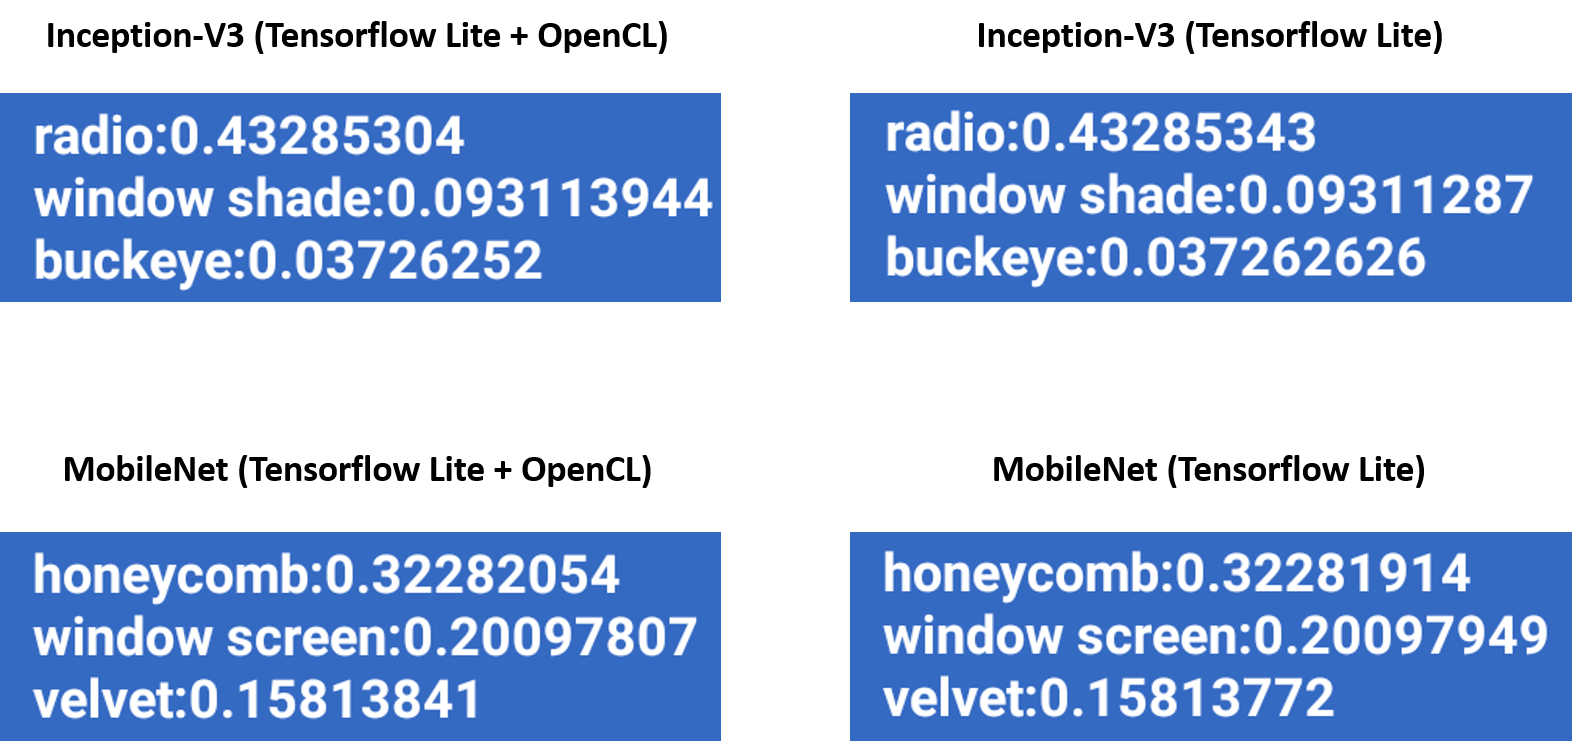
\includegraphics[width=0.75\textwidth]
	{pics/correct.png}
	\caption{Hasil pengujian terhadap keseluruhan proses \textit{inference} menggunakan aplikasi pengenalan citra yang diimplementasikan menggunakan Tensorflow Lite.}
	\label{fig:correct}
\end{figure}

%-----------------------------------------------------------------------------%
\section{Eksperimen Untuk Membandingkan Kecepatan \textit{Kernel} Operasi Perkalian Matriks-Matriks }
%-----------------------------------------------------------------------------%
Eksperimen ini bertujuan untuk menguji dan membandingkan kecepatan tiga jenis Tensorflow Lite \textit{kernel} untuk operasi perkalian matriks-matriks. Pada eksperimen ini digunakan ukuran yang sama untuk dua matriks masukan dan juga matriks keluaran. Terdapat lima variasi ukuran $tinggi \times lebar$ matriks yang diuji, yaitu $64 \times 64$, $128 \times 128$, $256 \times 256$, $512 \times 512$, dan $1024 \times 1024$. Dengan demikian, akan terlihat \textit{kernel} mana saja yang unggul dalam komputasi matriks kecil dan \textit{kernel} mana saja yang unggul dalam komputasi matriks besar. Selain itu pada eksperimen ini juga akan terlihat bagaimana transfer data antara memori CPU dan GPU berpengaruh terhadap kecepatan Tensorflow Lite \textit{kernel} untuk operasi perkalian matriks-matriks yang diimplementasikan menggunakan OpenCL. Akan diketahui \textit{bottleneck} dari program OpenCL pada matriks besar dan matriks kecil. Waktu eksekusi suatu \textit{kernel} diukur menggunakan satuan milidetik.

Hasil eksperimen terhadap kecepatan dari tiga jenis \textit{kernel} dapat dilihat pada \tab~\ref{tab:matmatmulspeed}. Nilai-nilai dari tabel tersebut dalah rata-rata (dalam milidetik) dari 10 kali eksekusi \textit{kernel}. Standar deviasi dari 10 eksekusi tersebut dapat dilihat pada \tab~\ref{tab:matmatmuldev}. Secara visual, perbandingan kecepatan antara ketiga jenis \textit{kernel} dapat dilihat pada \pic~\ref{fig:matmatmul}. 

\begin{table}
	\centering
	\caption{Hasil eksperimen terhadap Tensorflow Lite \textit{kernel} untuk operasi perkalian matriks-matriks, dimana nilai-nilai pada tabel adalah rata-rata dari 10 kali eksekusi dalam milidetik.}
	\label{tab:matmatmulspeed}
	\begin{tabular}{|>{\small}R{2.5cm}|>{\small}R{2.1cm}|>{\small}R{2.1cm}|>{\small}R{2.1cm}|>{\small}R{2.4cm}|}
		\hline
		\multicolumn{1}{|>{\small}L{2.5cm}|}{\textbf{Tinggi x Lebar Masukan}} & 
		\multicolumn{1}{>{\small}L{2.1cm}|}{\textbf{Naive Kernel}} & 
		\multicolumn{1}{>{\small}L{2.1cm}|}{\textbf{Optimized Kernel}} & 
		\multicolumn{1}{>{\small}L{2.1cm}|}{\textbf{OpenCL Kernel}} & 
		\multicolumn{1}{>{\small}L{2.4cm}|}{\textbf{OpenCL + Transfer Data}} \\
		\hline
		$64 \times 64$ & 4.3596 & 1.1243 & 1.5501 & 7.6569
		\\
		\hline
		$128 \times 128$ & 33.9033 & 7.7470 & 2.3841 & 8.6730
		\\
		\hline
		$256 \times 256$ & 205.9833 & 62.4273 & 14.2164 & 21.7435
		\\
		\hline
		$512 \times 512$ & 1193.9166 & 373.4296 & 107.3510 & 116.6284
		\\
		\hline
		$1024 \times 1024$ & 9518.9719 & 3507.8444 & 824.9642 & 848.4501
		\\
		\hline
	\end{tabular}
\end{table}

\begin{table}
	\centering
	\caption{Standar deviasi dari 10 kali eksekusi (dalam milidetik) Tensorflow Lite \textit{kernel} untuk operasi perkalian matriks-matriks.}
	\label{tab:matmatmuldev}
	\begin{tabular}{|>{\small}R{2.5cm}|>{\small}R{2.1cm}|>{\small}R{2.1cm}|>{\small}R{2.1cm}|>{\small}R{2.4cm}|}
	\hline
	\multicolumn{1}{|>{\small}L{2.5cm}|}{\textbf{Tinggi x Lebar Masukan}} & 
	\multicolumn{1}{>{\small}L{2.1cm}|}{\textbf{Naive Kernel}} & 
	\multicolumn{1}{>{\small}L{2.1cm}|}{\textbf{Optimized Kernel}} & 
	\multicolumn{1}{>{\small}L{2.1cm}|}{\textbf{OpenCL Kernel}} & 
	\multicolumn{1}{>{\small}L{2.4cm}|}{\textbf{OpenCL + Transfer Data}} \\
	\hline
		$64 \times 64$ & 0.0958 & 0.1270 & 0.0726 & 0.7545
		\\
		\hline
		$128 \times 128$ & 0.4717 & 0.7324 & 0.0504 & 1.0877
		\\
		\hline
		$256 \times 256$ & 4.5170 & 1.3869 & 0.0912 & 0.9902
		\\
		\hline
		$512 \times 512$ & 1.8006 & 3.3557 & 0.1832 & 0.8476
		\\
		\hline
		$1024 \times 1024$ & 3.1632 & 10.8558 & 0.1265 & 0.9315
		\\
		\hline
	\end{tabular}
\end{table}

\begin{figure}
	\centering
	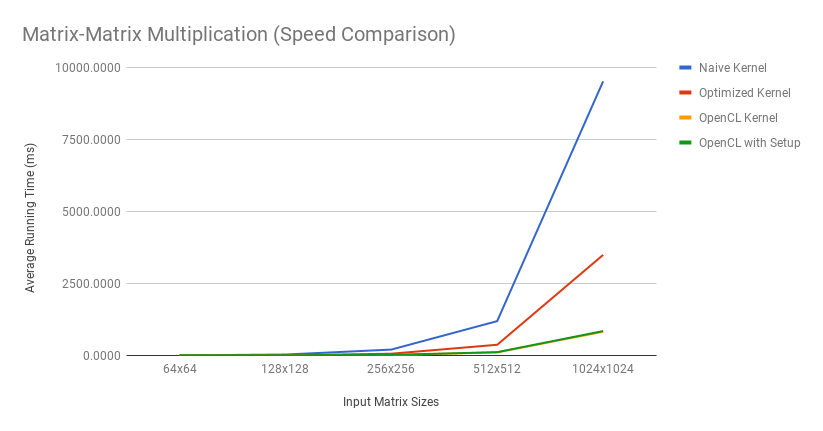
\includegraphics[width=0.75\textwidth]
	{pics/matmatmul.png}
	\caption{Perbandingan kecepatan tiga jenis \textit{kernel} untuk operasi perkalian matriks-matriks.}
	\label{fig:matmatmul}
\end{figure}

Dari hasil eksperimen di atas dapat dilihat bahwa Tensorflow Lite \textit{kernel} untuk operasi perkalian matriks-matriks yang berjalan di GPU melalui OpenCL memiliki kecepatan yang paling baik, terutama untuk matriks berukuran besar. Ketika hanya memperhatikan kecepatan OpenCL \textit{kernel} tanpa transfer data antar memori, OpenCL \textit{kernel} memiliki kecepatan yang lebih baik dari dua \textit{kernel} lain saat ukuran matriks $128 \times 128$ atau lebih besar. Sementara itu ketika transfer data antar memori dimasukkan ke dalam penghitungan, OpenCL \textit{kernel} baru mencapai kecepatan terbaik ketika ukuran matriks $256 \times 256$ atau lebih besar.

\section{Eksperimen Untuk Membandingkan Kecepatan \textit{Kernel} Operasi Konvolusi Matriks }
%-----------------------------------------------------------------------------%
Eksperimen ini bertujuan untuk menguji dan membandingkan kecepatan tiga jenis Tensorflow Lite \textit{kernel} untuk operasi konvolusi matriks. Pada eksperimen ini digunakan beberapa jenis ukuran matriks-matriks masukan dan matriks keluaran. Untuk operasi ini penulis membagi eksperimen ke dalam tiga kasus uji, antara lain kasus ketika ukuran $tinggi \times lebar$ matriks masukan bervariasi, kasus ketika kedalaman matriks masukan bervariasi, dan kasus ketika ukuran $kanal \times \textit{batch}$ matriks keluaran bervariasi. Pada eksperimen ini akan terlihat \textit{kernel} mana saja yang unggul dalam berbagai kasus yang diuji. Selain itu juga akan terlihat bagaimana transfer data antara memori CPU dan GPU berpengaruh terhadap kecepatan Tensorflow Lite \textit{kernel} untuk operasi konvolusi yang menggunakan OpenCL. Akan diketahui \textit{bottleneck} dari program OpenCL pada berbagai kasus uji. Waktu eksekusi suatu \textit{kernel} diukur menggunakan satuan milidetik.

\subsection{Konvolusi dengan Tinggi dan Lebar Matriks Masukan yang Bervariasi}
Pada eksperimen ini, diberikan matriks masukan dengan tinggi dan lebar yang bervariasi sehingga dapat diketahui bagaimana besar kecilnya ukuran tinggi dan lebar matriks masukan mempengaruhi kecepatan dari tiga jenis \textit{kernel}. Spesifikasi ukuran dari matriks masukan dan matriks filter yang digunakan dapat dilihat pada \tab~\ref{tab:imagefilterspec1}. Terdapat lima variasi ukuran $tinggi \times lebar$ matriks masukan yang diuji, yaitu $32 \times 32$, $64 \times 64$, $128 \times 128$, $256 \times 256$, dan $512 \times 512$. Dalam OpenCL, tinggi dan lebar dari matriks masukan terkait dengan tinggi dan lebar dari \textit{NDRange} yang digunakan dalam eksekusi OpenCL \textit{kernel}.

\begin{table}
	\centering
	\caption{Spesifikasi ukuran matriks masukan dan matriks filter yang diujikan untuk operasi konvolusi pada kasus tinggi dan lebar matriks masukan yang bervariasi.}
	\label{tab:imagefilterspec1}
	\begin{tabular}{|>{\small}L{2.1cm}|>{\small}L{2.1cm}|>{\small}L{2.1cm}|>{\small}L{2.1cm}|>{\small}L{2.4cm}|}
		\hline
		\textbf{Matriks} & \textbf{Kedalaman} & \textbf{Tinggi} & \textbf{Lebar} & \textbf{Banyak Batch} 
		\\
		\hline
		Masukan & 4 & bervariasi & bervariasi & 1
		\\
		\hline
		Filter & 4 & 5 & 5 & 4
		\\
		\hline
	\end{tabular}
\end{table}

Hasil eksperimen terhadap kecepatan dari tiga jenis \textit{kernel} pada kasus bervariasinya tinggi dan lebar matriks masukan ini dapat dilihat pada \tab~\ref{tab:convvarhwspeed}. Nilai-nilai dari tabel tersebut dalah rata-rata (dalam milidetik) dari 10 kali eksekusi \textit{kernel}. Standar deviasi dari 10 eksekusi tersebut dapat dilihat pada \tab~\ref{tab:convvarhwdev}. Secara visual, perbandingan kecepatan antara ketiga jenis \textit{kernel} dapat dilihat pada \pic~\ref{fig:convvarhw}.

\begin{table}
	\centering
	\caption{Hasil eksperimen terhadap Tensorflow Lite \textit{kernel} untuk operasi konvolusi matriks pada kasus ketika tinggi dan lebar matriks masukan bervariasi, dimana nilai-nilai pada tabel adalah rata-rata dari 10 kali eksekusi dalam milidetik.}
	\label{tab:convvarhwspeed}
\begin{tabular}{|>{\small}R{2.5cm}|>{\small}R{2.1cm}|>{\small}R{2.1cm}|>{\small}R{2.1cm}|>{\small}R{2.4cm}|}
	\hline
	\multicolumn{1}{|>{\small}L{2.5cm}|}{\textbf{Tinggi x Lebar Masukan}} & 
	\multicolumn{1}{>{\small}L{2.1cm}|}{\textbf{Naive Kernel}} & 
	\multicolumn{1}{>{\small}L{2.1cm}|}{\textbf{Optimized Kernel}} & 
	\multicolumn{1}{>{\small}L{2.1cm}|}{\textbf{OpenCL Kernel}} & 
	\multicolumn{1}{>{\small}L{2.4cm}|}{\textbf{OpenCL + Transfer Data}} \\
	\hline
		$32 \times 32$ & 6.6511 & 4.7852 & 1.5196 & 6.1364
		\\
		\hline
		$64 \times 64$ & 31.3152 & 13.4992 & 1.8377 & 7.9563
		\\
		\hline
		$128 \times 128$ & 113.8935 & 43.4996 & 5.5047 & 13.1798
		\\
		\hline
		$256 \times 256$ & 366.5030 & 122.3684 & 20.1672 & 31.9092
		\\
		\hline
		$512 \times 512$ & 1283.9716 & 401.0434 & 79.5439 & 111.8054
		\\
		\hline
	\end{tabular}
\end{table}

\begin{table}
	\centering
	\caption{Standar deviasi dari 10 kali eksekusi (dalam milidetik) Tensorflow Lite \textit{kernel} untuk operasi konvolusi matriks pada kasus ketika tinggi dan lebar matriks masukan bervariasi.}
	\label{tab:convvarhwdev}
\begin{tabular}{|>{\small}R{2.5cm}|>{\small}R{2.1cm}|>{\small}R{2.1cm}|>{\small}R{2.1cm}|>{\small}R{2.4cm}|}
	\hline
	\multicolumn{1}{|>{\small}L{2.5cm}|}{\textbf{Tinggi x Lebar Masukan}} & 
	\multicolumn{1}{>{\small}L{2.1cm}|}{\textbf{Naive Kernel}} & 
	\multicolumn{1}{>{\small}L{2.1cm}|}{\textbf{Optimized Kernel}} & 
	\multicolumn{1}{>{\small}L{2.1cm}|}{\textbf{OpenCL Kernel}} & 
	\multicolumn{1}{>{\small}L{2.4cm}|}{\textbf{OpenCL + Transfer Data}} \\
	\hline
		$32 \times 32$ & 0.4444 & 0.9186 & 0.1311 & 0.6996
		\\
		\hline
		$64 \times 64$ & 0.9173 & 2.5479 & 0.0799 & 1.3398
		\\
		\hline
		$128 \times 128$ & 6.9582 & 9.9099 & 0.2741 & 1.5212
		\\
		\hline
		$256 \times 256$ & 9.9799 & 4.9044 & 0.3141 & 1.8619
		\\
		\hline
		$512 \times 512$ & 10.8159 & 3.3544 & 0.1262 & 1.7571
		\\
		\hline
	\end{tabular}
\end{table}

\begin{figure}
	\centering
	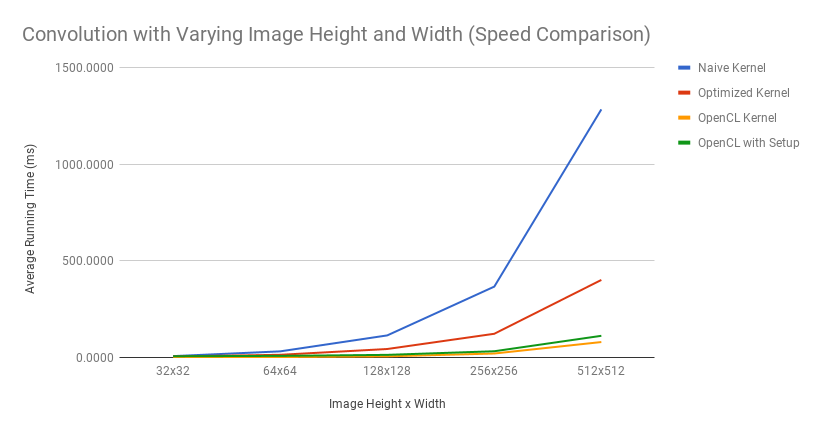
\includegraphics[width=0.75\textwidth]
	{pics/convvarhw.png}
	\caption{Perbandingan kecepatan tiga jenis \textit{kernel} untuk operasi konvolusi matriks pada kasus ketika tinggi dan lebar matriks masukan bervariasi.}
	\label{fig:convvarhw}
\end{figure}

Dari hasil eksperimen di atas dapat dilihat bahwa OpenCL \textit{kernel} untuk operasi konvolusi memiliki kecepatan yang paling baik. Ketika transfer data antar memori diabaikan, OpenCL \textit{kernel} \textit{kernel} memiliki kecepatan yang lebih baik dari dua \textit{kernel} lain pada semua variasi ukuran matriks yang diuji. Sementara itu ketika transfer data antar memori dimasukkan ke dalam penghitungan, OpenCL \textit{kernel} baru mencapai kecepatan terbaik saat $tinggi \times lebar$ dari matriks masukan berukuran $64 \times 64$ atau lebih besar.

\subsection{Konvolusi dengan Kedalaman Matriks Masukan yang Bervariasi}
Pada eksperimen ini, diberikan matriks masukan dengan kedalaman yang bervariasi sehingga dapat diketahui bagaimana banyak sedikitnya kanal dari matriks masukan mempengaruhi kecepatan dari tiga jenis \textit{kernel}. Spesifikasi ukuran dari matriks masukan dan matriks filter yang digunakan dapat dilihat pada \tab~\ref{tab:imagefilterspec2}. Terdapat lima variasi kedalaman matriks masukan yang diuji, yaitu $64$, $128$, $256$, $512$, dan $1024$. Dalam OpenCL, kedalaman dari matriks masukan terkait dengan banyaknya iterasi ketika melakukan konvolusi pada setiap \textit{work-item}. Semakin besar ukuran kanal dari matriks masukan, semakin besar pula beban komputasi pada setiap \textit{work-item}.

\begin{table}
	\centering
	\caption{Spesifikasi ukuran matriks masukan dan matriks filter yang diujikan untuk operasi konvolusi pada kasus kedalaman dari matriks masukan yang bervariasi.}
	\label{tab:imagefilterspec2}
\begin{tabular}{|>{\small}L{2.1cm}|>{\small}L{2.1cm}|>{\small}L{2.1cm}|>{\small}L{2.1cm}|>{\small}L{2.4cm}|}
	\hline
	\textbf{Matriks} & \textbf{Kedalaman} & \textbf{Tinggi} & \textbf{Lebar} & \textbf{Banyak Batch} 
		\\
		\hline
		Masukan & bervariasi & 16 & 16 & 1
		\\
		\hline
		Filter & bervariasi & 5 & 5 & 4
		\\
		\hline
	\end{tabular}
\end{table}

Hasil eksperimen terhadap kecepatan dari tiga jenis \textit{kernel} dalam kasus bervariasinya kedalaman matriks masukan ini dapat dilihat pada \tab~\ref{tab:convvarchnspeed}. Nilai-nilai dari tabel tersebut dalah rata-rata (dalam milidetik) dari 10 kali eksekusi \textit{kernel}. Standar deviasi dari 10 eksekusi tersebut dapat dilihat pada \tab~\ref{tab:convvarchndev}. Secara visual, perbandingan kecepatan antara ketiga jenis \textit{kernel} dapat dilihat pada \pic~\ref{fig:convvarchn}.

\begin{table}
	\centering
	\caption{Hasil eksperimen terhadap Tensorflow Lite \textit{kernel} untuk operasi konvolusi pada kasus ketika kedalaman matriks masukan bervariasi, dimana nilai-nilai pada tabel adalah rata-rata dari 10 kali eksekusi dalam milidetik.}
	\label{tab:convvarchnspeed}
\begin{tabular}{|>{\small}R{2.5cm}|>{\small}R{2.1cm}|>{\small}R{2.1cm}|>{\small}R{2.1cm}|>{\small}R{2.4cm}|}
	\hline
	\multicolumn{1}{|>{\small}L{2.5cm}|}{\textbf{Kedalaman Masukan}} & 
	\multicolumn{1}{>{\small}L{2.1cm}|}{\textbf{Naive Kernel}} & 
	\multicolumn{1}{>{\small}L{2.1cm}|}{\textbf{Optimized Kernel}} & 
	\multicolumn{1}{>{\small}L{2.1cm}|}{\textbf{OpenCL Kernel}} & 
	\multicolumn{1}{>{\small}L{2.4cm}|}{\textbf{OpenCL + Transfer Data}} \\
	\hline
		64 & 12.4833 & 12.8914 & 1.6086 & 9.1080
		\\
		\hline
		128 & 24.3573 & 24.1618 & 2.8356 & 9.9595
		\\
		\hline
		256 & 52.3216 & 51.8085 & 5.0332 & 13.4032
		\\
		\hline
		512 & 85.7740 & 92.0345 & 8.6298 & 15.9954
		\\
		\hline
		1024 & 152.1905 & 165.9758 & 19.0146 & 26.8229
		\\
		\hline
	\end{tabular}
\end{table}

\begin{table}
	\centering
	\caption{Standar deviasi dari 10 kali eksekusi (dalam milidetik) Tensorflow Lite \textit{kernel} untuk operasi konvolusi matriks pada kasus ketika kedalaman matriks masukan bervariasi.}
	\label{tab:convvarchndev}
\begin{tabular}{|>{\small}R{2.5cm}|>{\small}R{2.1cm}|>{\small}R{2.1cm}|>{\small}R{2.1cm}|>{\small}R{2.4cm}|}
	\hline
	\multicolumn{1}{|>{\small}L{2.5cm}|}{\textbf{Kedalaman Masukan}} & 
	\multicolumn{1}{>{\small}L{2.1cm}|}{\textbf{Naive Kernel}} & 
	\multicolumn{1}{>{\small}L{2.1cm}|}{\textbf{Optimized Kernel}} & 
	\multicolumn{1}{>{\small}L{2.1cm}|}{\textbf{OpenCL Kernel}} & 
	\multicolumn{1}{>{\small}L{2.4cm}|}{\textbf{OpenCL + Transfer Data}} \\
	\hline
		64 & 1.2069 & 1.0923 & 0.0874 & 1.1450
		\\
		\hline
		128 & 2.2827 & 1.9532 & 0.3127 & 1.4827
		\\
		\hline
		256 & 1.8923 & 4.9887 & 0.5981 & 1.8302
		\\
		\hline
		512 & 6.2608 & 3.8101 & 0.1258 & 0.8930
		\\
		\hline
		1024 & 2.0152 & 9.3311 & 0.2196 & 0.9503
		\\
		\hline
	\end{tabular}
\end{table}

\begin{figure}
	\centering
	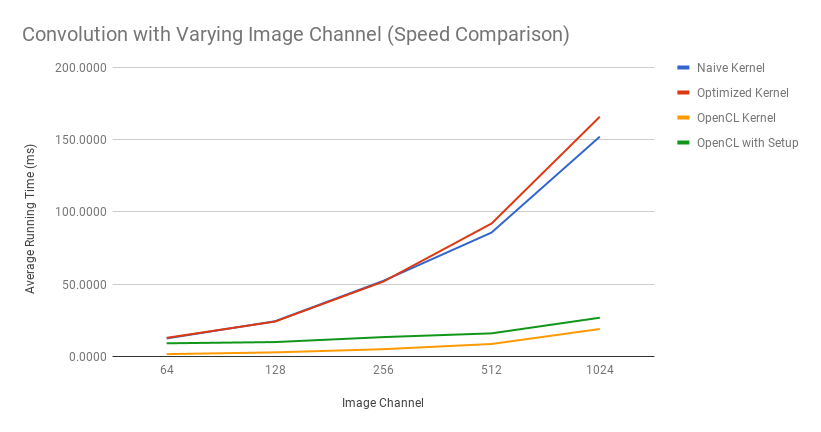
\includegraphics[width=0.75\textwidth]
	{pics/convvarchn.png}
	\caption{Perbandingan kecepatan tiga jenis \textit{kernel} untuk operasi konvolusi matriks pada kasus ketika kedalaman matriks masukan bervariasi.}
	\label{fig:convvarchn}
\end{figure}

Dari hasil eksperimen di atas dapat dilihat bahwa Tensorflow Lite \textit{kernel} untuk operasi konvolusi yang berjalan di GPU melalui OpenCL memiliki kecepatan yang paling baik. Ketika waktu untuk transfer data antara memori CPU dan GPU diperhitungkan maupun ketika tidak diperhitungkan, OpenCL \textit{kernel} memiliki kecepatan yang lebih baik dari dua \textit{kernel} lainnya pada semua variasi ukuran matriks yang diuji.

\subsection{Konvolusi dengan Banyaknya \textit{Batch} dan Kedalaman Matriks Masukan yang Bervariasi}
Pada eksperimen ini, diberikan matriks masukan dan matriks filter dengan \textit{batch} yang bervariasi. Banyaknya \textit{batch} dari matriks masukan sama dengan banyaknya \textit{batch} dari matriks keluaran, sedangkan banyaknya \textit{batch} dari matriks filter sama dengan kedalaman dari matriks keluaran. Pada eksperimen ini ingin diketahui bagaimana banyak sedikitnya \textit{batch} dan kanal dari matriks keluaran mempengaruhi kecepatan tiga jenis kernel \textit{kernel}. Spesifikasi ukuran dari matriks masukan dan matriks filter yang digunakan dapat dilihat pada \tab~\ref{tab:imagefilterspec3}. Terdapat lima variasi ukuran $tinggi \times lebar$ matriks masukan yang diuji, yaitu $8 \times 8$, $16 \times 16$, $32 \times 32$, $64 \times 64$, dan $128 \times 128$. Dalam OpenCL, banyaknya \textit{batch} dan kanal dari matriks keluaran terkait dengan lebar dan tinggi dari \textit{NDRange} yang digunakan dalam eksekusi OpenCL \textit{kernel}.

\begin{table}
	\centering
	\caption{Spesifikasi ukuran matriks masukan dan matriks filter yang diujikan untuk operasi konvolusi pada kasus banyaknya \textit{batch} dan \textit{kanal} dari matriks keluaran yang bervariasi.}
	\label{tab:imagefilterspec3}
\begin{tabular}{|>{\small}L{2.1cm}|>{\small}L{2.1cm}|>{\small}L{2.1cm}|>{\small}L{2.1cm}|>{\small}L{2.4cm}|}
	\hline
	\textbf{Matriks} & \textbf{Kedalaman} & \textbf{Tinggi} & \textbf{Lebar} & \textbf{Banyak Batch} 
		\\
		\hline
		Image & 4 & 16 & 16 & bervariasi
		\\
		\hline
		Filter & 4 & 5 & 5 & bervariasi
		\\
		\hline
	\end{tabular}
\end{table}

Hasil eksperimen terhadap kecepatan dari tiga jenis \textit{kernel} pada kasus bervariasinya banyak \textit{batch} dan kanal matriks keluaran ini dapat dilihat pada \tab~\ref{tab:convvarbchnspeed}. Nilai-nilai dari tabel tersebut dalah rata-rata (dalam milidetik) dari 10 kali eksekusi \textit{kernel}. Standar deviasi dari 10 eksekusi tersebut dapat dilihat pada \tab~\ref{tab:convvarbchndev}. Secara visual, perbandingan kecepatan antara ketiga jenis \textit{kernel} dapat dilihat pada \pic~\ref{fig:convvarbchn}.

\begin{table}
	\centering
	\caption{Hasil eksperimen terhadap Tensorflow Lite \textit{kernel} untuk operasi konvolusi matriks pada kasus ketika banyaknya \textit{batch} dan kanal matriks keluaran bervariasi, dimana nilai-nilai pada tabel adalah rata-rata dari 10 kali eksekusi dalam milidetik.}
	\label{tab:convvarbchnspeed}
\begin{tabular}{|>{\small}R{2.5cm}|>{\small}R{2.1cm}|>{\small}R{2.1cm}|>{\small}R{2.1cm}|>{\small}R{2.4cm}|}
	\hline
	\multicolumn{1}{|>{\small}L{2.5cm}|}{\textbf{Banyak Batch x Kedalaman Masukan}} & 
	\multicolumn{1}{>{\small}L{2.1cm}|}{\textbf{Naive Kernel}} & 
	\multicolumn{1}{>{\small}L{2.1cm}|}{\textbf{Optimized Kernel}} & 
	\multicolumn{1}{>{\small}L{2.1cm}|}{\textbf{OpenCL Kernel}} & 
	\multicolumn{1}{>{\small}L{2.4cm}|}{\textbf{OpenCL + Transfer Data}} \\
	\hline
		$8 \times 8$ & 21.3206 & 6.8149 & 1.7034 & 9.6239
		\\
		\hline
		$16 \times 16$ & 77.6343 & 11.5020 & 4.5229 & 12.9872
		\\
		\hline
		$32 \times 32$ & 241.5599 & 20.3202 & 15.9239 & 24.1819
		\\
		\hline
		$64 \times 64$ & 756.2591 & 44.4415 & 61.0587 & 75.0377
		\\
		\hline
		$128 \times 128$ & 2847.1164 & 106.8449 & 236.1338 & 262.0281
		\\
		\hline
	\end{tabular}
\end{table}

\begin{table}
	\centering
	\caption{Standar deviasi dari 10 kali eksekusi (dalam milidetik) Tensorflow Lite \textit{kernel} untuk operasi konvolusi matriks pada kasus ketika banyaknya \textit{batch} dan kanal matriks keluaran bervariasi.}
	\label{tab:convvarbchndev}
\begin{tabular}{|>{\small}R{2.5cm}|>{\small}R{2.1cm}|>{\small}R{2.1cm}|>{\small}R{2.1cm}|>{\small}R{2.4cm}|}
	\hline
	\multicolumn{1}{|>{\small}L{2.5cm}|}{\textbf{Banyak Batch x Kedalaman Masukan}} & 
	\multicolumn{1}{>{\small}L{2.1cm}|}{\textbf{Naive Kernel}} & 
	\multicolumn{1}{>{\small}L{2.1cm}|}{\textbf{Optimized Kernel}} & 
	\multicolumn{1}{>{\small}L{2.1cm}|}{\textbf{OpenCL Kernel}} & 
	\multicolumn{1}{>{\small}L{2.4cm}|}{\textbf{OpenCL + Transfer Data}} \\
	\hline
		$8 \times 8$ & 2.4153 & 0.6333 & 0.1556 & 1.5570
		\\
		\hline
		$16 \times 16$ & 4.3455 & 1.6288 & 0.2239 & 1.4405
		\\
		\hline
		$32 \times 32$ & 7.2629 & 1.5248 & 0.1507 & 1.0567
		\\
		\hline
		$64 \times 64$ & 3.0043 & 1.2937 & 0.0650 & 2.5150
		\\
		\hline
		$128 \times 128$ & 8.1991 & 7.3458 & 0.6611 & 10.9892
		\\
		\hline
	\end{tabular}
\end{table}

\begin{figure}
	\centering
	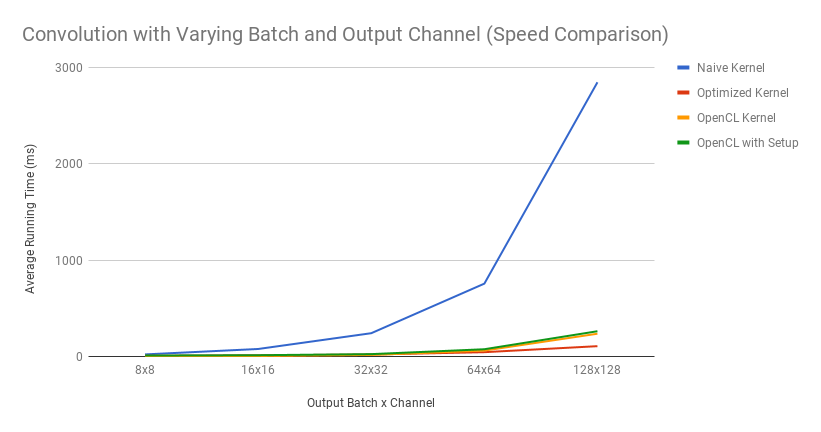
\includegraphics[width=0.75\textwidth]
	{pics/convvarbchn.png}
	\caption{Perbandingan kecepatan tiga jenis \textit{kernel} untuk operasi konvolusi matriks pada kasus ketika banyaknya \textit{batch} dan kanal matriks keluaran bervariasi.}
	\label{fig:convvarbchn}
\end{figure}

Dari hasil eksperimen di atas dapat dilihat bahwa Tensorflow Lite \textit{optimized kernel} yang berjalan di CPU memiliki kecepatan yang paling baik ketika ukuran matriks keluaran semakin besar. \textit{Optimized kernel} mampu mengungguli kecepatan OpenCL \textit{kernel} tanpa menghitung transfer data antar memori ketika $batch \times kanal$ dari matriks keluaran berukuran $64 \times 64$ atau lebih besar. \textit{Optimized kernel} juga mampu mengungguli kecepatan OpenCL \textit{kernel} pada semua variasi ukuran matriks keluaran yang diuji ketika transfer data antara memori CPU dan GPU diperhitungkan.

%-----------------------------------------------------------------------------%
\section{Analisis }
%-----------------------------------------------------------------------------%
Dari hasil eksperimen yang telah dilakukan dapat dilihat bahwa Tensoflow Lite yang telah ditambahkan dengan OpenCL \textit{kernel} yang berjalan di GPU dapat menghasilkan keluaran yang sesuai ketika melakukan proses \textit{inference} menggunakan dua jenis model CNN yang diuji. Jika di perhatikan, Tensorflow Lite yang telah ditambahkan dengan OpenCL \textit{kernel} menghasilkan keluaran yang sama dengan Tensorflow Lite tanpa modifikasi hingga lima angka di belakang koma. Sedikit perbedaan pada hasil dari proses inference ini dapat disebabkan oleh galat dalam pembulatan angka. Karena \textit{kernel} yang digunakan berbeda, maka langkah-langkah komputasi yang dilakukan oleh prosesor juga berbeda. Hal ini dapat menyebabkan hasil akhir sedikit berbeda karena galat pembulatan yang berbeda pada setiap langkah komputasi dan terus terakumulasi hingga akhir komputasi.

Dari hasil eksperimen yang telah dilakukan juga dapat dilihat bahwa Tensorflow Lite \textit{kernel} yang berjalan di GPU melalui OpenCL memiliki kecepatan yang cukup baik. OpenCL \textit{kernel} selalu dapat mengungguli kecepatan \textit{naive kernel} dari Tensorflow Lite yang berjalan di CPU pada semua kasus uji baik pada operasi perkalian matriks-matriks maupun konvolusi matriks. OpenCL \textit{kernel} juga mampu mengungguli kecepatan \textit{optimized kernel} pada operasi perkalian matriks-matriks ketika ukuran matriks cukup besar. Pada operasi konvolusi matriks, kecepatan OpenCL \textit{kernel} mampu bersaing dengan \textit{optimized kernel} meskipun terdapat kasus dimana kecepatan OpenCL \textit{kernel} tidak mampu mengungguli kecepatan \textit{optimized kernel}. Hal ini cukup sesuai dengan dugaan awal bahwa operasi-operasi matriks yang diimplementasikan menggunakan paradigma pemrograman paralel dan dijalankan di GPU dapat memiliki kecepatan komputasi yang sangat baik. 

Berbeda dengan CPU yang pada umumnya hanya memiliki mepat hingga delapan \textit{cores}, GPU memiliki ratusan \textit{core} yang sangat mendukung komputasi secara paralel sehingga memiliki performa komputasi yang tinggi. Komputasi secara paralel lebih efisien daripada komputasi sekuensial karena \textit{chips} pada perangkat keras pada dasarnya bersifat paralel. \textit{Chips} mengandung miliaran transistor. Prosesor dengan banyak \textit{core} seperti GPU mengatur transistor-transistor menjadi banyak prosesor paralel yang mengandung ratusan unit komputasi \textit{floating point}. Kemampuan GPU bukan satu-satunya faktor yang meningkatkan performa komputasi, program yang diimplementasikan secara paralel dengan baik juga menjadi faktor dalam meningkatnya kecepatan komputasi. Dalam hal ini OpenCL menyediakan model pemrograman paralel yang baik sehingga mendukung implementasi program paralel yang memiliki performa tinggi \cite{openclguide}. 

Terdapat dua kasus uji pada eksperimen yang perlu diperhatikan, yaitu ketika tinggi dan lebar matriks masukan bervariasi dan ketika banyaknya \textit{batch} dan kanal matriks keluaran bervariasi. Perhatikan bahwa bertambahnya tinggi dan lebar matriks masukan dan bertambahnya \textit{batch} dan kanal matriks keluaran sama-sama berdampak pada bertambahnya tinggi dan lebar \textit{NDRange}. Artinya, bertambahnya tinggi dan lebar matriks masukan dan bertambahnya \textit{batch} dan kanal matriks keluaran memiliki dampak yang sama terhadap kecepatan OpenCL \textit{kernel}. Dari hasil eksperimen diperoleh bahwa pada saat tinggi dan lebar matriks masukan berukuran besar, kecepatan OpenCL \textit{kernel} mampu mengungguli \textit{optimized kernel}, namun pada saat \textit{batch} dan kanal matriks keluaran berukuran besar, kecepatan \textit{optimized kernel} justru mengungguli OpenCL \textit{kernel}. Hal ini terjadi karena kenaikan waktu eksekusi \textit{optimized kernel} akibat membesarnya \textit{batch} dan kanal matriks keluaran jauh lebih kecil daripada kenaikan waktu eksekusi \textit{optimized kernel} akibat membesarnya tinggi dan lebar matriks masukan.

Penjelasan di atas dapat dibuktikan menggunakan eksperimen tambahan. Pada eksperimen ini penulis membandingkan kecepatan eksekusi pada dua matriks dengan spesifikasi seperti pada \tab~\ref{tab:hwvsbc1} dan \tab~\ref{tab:hwvsbc2}. Pada matriks pertama, tinggi dan lebar matriks masukan berukuran besar. Ukuran $tinggi \times lebar$ \textit{NDRange} yang digunakan oleh OpenCL \textit{kernel} untuk matriks tersebut adalah $(1 \times 512) \times (512 \times 4 / 4) = 512 \times 512$. Pada matriks kedua, \textit{batch} dan kanal matriks keluaran cukup berukuran besar. Ukuran $tinggi \times lebar$ \textit{NDRange} yang digunakan oleh OpenCL \textit{kernel} untuk matriks tersebut adalah $(32 \times 16) \times (16 \times 128 / 4) = 512 \times 512$. Kedua matriks tersebut memunculkan ukuran \textit{NDRange} yang sama, sehingga kecepatan eksekusi OpenCL \textit{kernel} seharusnya sama. Hal ini dapat dilihat pada \tab~\ref{tab:hwvsbcspeed}. Terlihat bahwa OpenCL \textit{kernel} memiliki kecepatan yang kurang lebih sama pada kedua jenis matriks masukan, sedangkan kecepatan \textit{optimized kernel} jauh lebih baik ketika \textit{batch} dan kanal matriks keluaran berukuran besar.

\begin{table}
	\centering
	\caption{Spesifikasi matriks pertama yang memiliki tinggi dan lebar matriks masukan yang berukuran besar.}
	\label{tab:hwvsbc1}
\begin{tabular}{|>{\small}L{2.1cm}|>{\small}L{2.1cm}|>{\small}L{2.1cm}|>{\small}L{2.1cm}|>{\small}L{2.4cm}|}
	\hline
	\textbf{Matriks} & \textbf{Kedalaman} & \textbf{Tinggi} & \textbf{Lebar} & \textbf{Banyak Batch} 
		\\
		\hline
		Image & 4 & 516 & 516 & 1
		\\
		\hline
		Filter & 4 & 5 & 5 & 4
		\\
		\hline
		Output & 4 & 512 & 512 & 1
		\\
		\hline
	\end{tabular}
\end{table}

\begin{table}
	\centering
	\caption{Spesifikasi matriks kedua yang memiliki \textit{batch} dan kanal matriks keluaran yang banyak.}
	\label{tab:hwvsbc2}
\begin{tabular}{|>{\small}L{2.1cm}|>{\small}L{2.1cm}|>{\small}L{2.1cm}|>{\small}L{2.1cm}|>{\small}L{2.4cm}|}
	\hline
	\textbf{Matriks} & \textbf{Kedalaman} & \textbf{Tinggi} & \textbf{Lebar} & \textbf{Banyaknya Batch} 
		\\
		\hline
		Image & 4 & 20 & 20 & 32
		\\
		\hline
		Filter & 4 & 5 & 5 & 128
		\\
		\hline
		Output & 128 & 16 & 16 & 32
		\\
		\hline
	\end{tabular}
\end{table}

\begin{table}
	\centering
	\caption{Hasil perbandingan kecepatan Tensorflow Lite \textit{kernel} pada dua jenis matriks masukan, dimana nilai-nilai pada tabel adalah rata-rata dari 10 kali eksekusi dalam milidetik.}
	\label{tab:hwvsbcspeed}
\begin{tabular}{|>{\small}R{2.5cm}|>{\small}R{2.1cm}|>{\small}R{2.1cm}|>{\small}R{2.1cm}|>{\small}R{2.4cm}|}
	\hline
	\multicolumn{1}{|>{\small}L{2.5cm}|}{\textbf{Ukuran Keluaran}} & 
	\multicolumn{1}{>{\small}L{2.1cm}|}{\textbf{Naive Kernel}} & 
	\multicolumn{1}{>{\small}L{2.1cm}|}{\textbf{Optimized Kernel}} & 
	\multicolumn{1}{>{\small}L{2.1cm}|}{\textbf{OpenCL Kernel}} & 
	\multicolumn{1}{>{\small}L{2.4cm}|}{\textbf{OpenCL + Transfer Data}} \\
	\hline
		$Tinggi \times Lebar = 512 \times 512$ & 1300.6688 & 431.8264 & 79.6208 & 107.6360
		\\
		\hline
		$Banyak Batch \times Kedalaman = 32 \times 128$ & 1301.6718 & 55.8074 & 79.6087 & 96.9623
		\\
		\hline
	\end{tabular}
\end{table}

Dalam penelitian ini, \textit{optimized kernel} hanya digunakan sebagai pembanding terhadap OpenCL \textit{kernel} yang telah diimplementasikan oleh penulis. Penulis tidak mempelajari algoritma yang digunakan dalam implementasi \textit{optimized kernel} secara mendalam. Analisis terhadap alasan mengapa \textit{optimized kernel} memiliki kecepatan yang lebih baik saat \textit{batch} dan kanal matriks keluaran berukuran besar daripada saat tinggi dan lebar matriks masukan berukuran besar berada diluar lingkup penelitian. Namun, menurut penulis alasan utama kecepatan OpenCL \textit{kernel} tidak dapat mengungguli kecepatan \textit{optimized kernel} pada beberapa kasus adalah karena operasi baca/tulis terhadap memori GPU hampir selalu menjadi \textit{bottleneck} dalam suatu OpenCL \textit{kernel} \cite{adrenoopencl}. Komputasi bukanlah penyebab lambatnya suatu OpenCL \textit{kernel} karena telah dijelaskan bahwa GPU memiliki performa komputasi yang sangat tinggi.

Pada semua kasus pengujian, dapat terlihat bahwa transfer data antara memori CPU dan GPU sangat mempengaruhi kecepatan OpenCL \textit{kernel} pada matriks-matriks yang berukuran kecil. Perhatikan bahwa pada semua kasus uji, transfer data antara memori GPU dan CPU menjadi \textit{bottleneck} ketika matriks berukuran kecil. Pada tabel hasil eksperimen, waktu yang diperlukan untuk transfer data antara memori CPU dan GPU adalah selisih antara waktu eksekusi OpenCL \textit{kernel} saja dengan waktu eksekusi OpenCL \textit{kernel} ditambah transfer data antara memori CPU dan GPU (selisih antara kolom keempat dan kolom kelima). Dapat dilihat bahwa selisih tersebut lebih besar daripada waktu eksekusi OpenCL \textit{kernel} saja ketika matriks-matriks yang terlibat berukuran relatif kecil. 

Pada matriks-matriks besar, transfer data antara memori CPU dan GPU tidak menjadi \textit{bottleneck}. Hal ini disebabkan oleh dua hal. Pertama, beban komputasi lebih berat ketika matriks berukuran besar. Kedua, beban untuk operasi baca/tulis terhadap memori GPU lebih juga berat ketika ukuran matriks semakin besar. Telah dijelaskan sebelumnya bahwa operasi baca/tulis terhadap memori GPU sering menjadi \textit{bottleneck} dari suatu OpenCL \textit{kernel}. Operasi baca/tulis tersebut memiliki peran lebih besar terhadap meningkatnya waktu eksekusi OpenCL \textit{kernel}. Jadi, operasi baca/tulis terhadap memori GPU pada OpenCL \textit{kernel} memiliki peran yang besar terhadap berpindahnya \textit{bottleneck} dari transfer data antar memori ke eksekusi OpenCL \textit{kernel}.